\documentclass[12pt,answers]{exam}

\usepackage{tikz, pgfplots}
\usepackage{amsmath}
\usepackage{hyperref}
\usepackage[empty]{fullpage}

\newcounter{countA}


\begin{document}
\subsection*{Midterm 2 Suggested Review Problems} 

Here are problems that are similar to the ones you might see on the
exam. Be sure to also review old quiz and workshop questions too.

\subsubsection*{Experiments vs.~Observational
Studies}\label{experiments-vs.-observational-studies}

Know the difference between explanatory variables, response variables,
and lurking variables. Also, make sure that you understand why
randomized controlled experiments let you establish cause and effect but
observational studies do not.


\begin{questions}
\setcounter{question}{\value{countA}}
\item A NY Times article titled \emph{Risks: Smokers Found More Prone to Dementia} states the following:

\begin{quote}
``Researchers analyzed data from 23,123 health plan members who
participated in a voluntary exam and health behavior survey from 1978 to
1985, when they were 50-60 years old. 23 years later, about 25\% of the
group had dementia, including 1,136 with Alzheimer's disease and 416
with vascular dementia. After adjusting for other factors, the
researchers concluded that pack-a-day smokers were 37\% more likely than
nonsmokers to develop dementia, and the risks went up with increased
smoking; 44\% for one to two packs a day; and twice the risk for more
than two packs.''
\end{quote}

\begin{parts}
\item
  Was this an experiment or an observational study? Why?
\begin{solution}
It's an observation study because there was no treatment imposed on the individuals. 
\end{solution}
\vfill
\item
  What are the explanatory and response variables?
\begin{solution}
Explanatory: smoking frequency (packs per day), Response: whether they have dementia.
\end{solution}
\vfill
\item
  Based on this study, can we conclude that smoking causes dementia
  later in life? Explain your reasoning.
\vfill
\begin{solution}
No, you can't prove cause \& effect with an observational study. There might be lurking variables like diet, exercise, income, etc. that are the real cause of the correlation. 
\end{solution}
\end{parts}


\question
  In a public health study on the effects of consumption of fruits and
  vegetables on psychological well-being in young adults, participants
  were randomly assigned to three groups: (1) diet as usual, (2) an
  intervention involving text message reminders to increase their fruits
  and vegetable consumption plus a voucher to purchase them, or (3) a
  fruit and vegetable intervention in which participants were given two
  additional daily servings of fresh fruits and vegetables to consume on
  top of their normal diet. Participants were asked to take a nightly
  survey on their smartphones. Participants were student volunteers at
  the University of Otago, New Zealand. At the end of the 14-day study,
  only participants in the third group showed improvements to their
  psychological well-being across the 14-days relative to the other
  groups.

\begin{parts}
\item
  What type of study is this?
\begin{solution}
This was an experiment.
\end{solution}
\vfill
\item
  Identify the explanatory and response variables.
\begin{solution}
Explanatory: treatment group (or fruit and vegetable consumption).  Response: psychological well-being.
\end{solution}
\vfill

\item
  Were the individuals in the study a random sample from the
  population?
\begin{solution}
No, they were student volunteers at one university.
\end{solution}
\vfill
\item
  Were the individuals randomly assigned to different treatment
  groups?
\begin{solution}
Yes.
\end{solution}
\vfill
\item
  Does this study support the claim that giving young adults fresh
  fruits and vegetables to eat can \emph{cause} psychological benefits?
\begin{solution}
Yes! You can establish cause and effect with a randomized controlled experiment like this one.
\end{solution}
\end{parts}
\setcounter{countA}{\value{question}}
\end{questions}

\subsubsection*{Probability}\label{probability}
\begin{questions}
\setcounter{question}{\value{countA}}
%\question (\href{https://people.hsc.edu/faculty-staff/blins/books/OpenIntroStats4e.pdf#eoce.3.5}{Exercise 3.5 OpenIntro Statistics})
%  If you flip a fair coin 10 times, what is the probability of
%
%  \begin{parts}
%  \item
%    getting all tails?
%\begin{solution}
%$$(1/2)^{10} = 0.0009765625 \text{ or } 0.098 \%.$$
%\end{solution}
%\vfill
%  \item
%    getting all heads?
%\begin{solution}
%$$(1/2)^{10} = 0.0009765625 \text{ or } 0.098 \%.$$
%\end{solution}
%\vfill
%  \item
%    getting at least one tails?
%\begin{solution}
%$$100\% - 0.098 \% = 99.9\%.$$
%\end{solution}
%\vfill
%  \end{parts}
%\question
%  A Pew Research survey asked 2,373 randomly sampled registered voters
%  their political affiliation (Republican, Democrat, or Independent) and
%  whether or not they identify as swing voters. 35\% of respondents
%  identified as Independent, 23\% identified as swing voters, and 11\%
%  identified as both.
%
%  \begin{parts}
%  \item
%    Are being Independent and being a swing voter disjoint,
%    i.e.~mutually exclusive?
%\begin{solution}
%No, because some voters are both.
%\end{solution}
%\vfill
%  \item
%    Are being Independent and being a swing voter independent events.
%    Hint: if they were independent, then you could use the
%    multiplication rule to calculate the probability that someone is
%    both a swing voter and a political Independent. Does the
%    multiplication rule give the correct answer?
%\begin{solution}
%They are not independent because if they were, the multiplication rule would tell us that the probability that some one is both a political Independent and a swing voters would be 
%$$(0.35)(0.23) = 8.05\%$$
%but the actual percent who are both is 11\%.  
%\end{solution}
%\vfill
%  \end{parts}
\question
  Data collected at elementary schools in DeKalb County, GA suggest that
  each year roughly 25\% of students miss exactly one day of school,
  15\% miss 2 days, and 28\% miss 3 or more days due to sickness.

  \begin{parts}
  \item
    What is the probability that a student chosen at random doesn't miss
    any days of school due to sickness this year?
\begin{solution}
Let $X$ represent the number of days a kid misses school.
$$P(X = 0) = 100\% - 25\% - 15\% - 28\% = 32\%.$$
\end{solution}
\vfill
  \item
    What is the probability that a student chosen at random misses no
    more than one day?
\begin{solution}
$$P(X \le 1) = 32\% + 25\% = 57\%.$$
\end{solution}
\vfill
  \item
    What is the probability that a student chosen at random misses at
    least one day?
\begin{solution}
$$P(X \ge 1) = 100\% - 32\% = 68\%.$$
\end{solution}
%  \item
%    If a parent has two kids at a DeKalb County elementary school, what
%    is the probability that neither kid will miss any school? Note any
%    assumption you must make to answer this question.
%\begin{solution}
%Let $X$ and $Y$ represent the number of days the two kids miss.
%If you assume that $X$ and $Y$ are independent, then 
%$$P(X = 0 \text{ and } Y = 0) = (0.32) (0.32) = 10.24\%.$$
%\end{solution}
%\vfill
%  \item
%    If a parent has two kids at a DeKalb County elementary school, what
%    is the probability that both kids will miss some school, i.e.~at
%    least one day? Note any assumption you make.
%\begin{solution}
%If you assume that the number of days each kid misses are independent, then 
%$$P(X \ge 1 \text{ and } Y \ge 1) = (0.68) (0.68) = 46.24\%.$$
%\end{solution}
%\vfill
  \end{parts}

\setcounter{countA}{\value{question}}
\end{questions}

\subsubsection*{Weighted Averages and Expected
Value}\label{weighted-averages-and-expected-value}

Expected value (also known as the theoretical average) is the weighted
average of the outcomes in a probability model. Make sure you understand
why it is called ``expected'' and how to calculate it. You should know
the Law of Large Numbers too.

\begin{questions}
\setcounter{question}{\value{countA}}

\item
  Andy is always looking for ways to make money fast. Lately, he has
  been trying to make money by gambling. Here is the game he is
  considering playing: The game costs \$2 to play. He draws a card from
  a deck. If he gets a number card (2-10), he wins nothing. For any face
  card ( jack, queen or king), he wins \$3. For any ace, he wins \$5,
  and he wins an extra \$20 if he draws the ace of clubs.

  \begin{parts}
  \item
    Create a probability model for this game.
\begin{solution}
\begin{center}
  \renewcommand{\arraystretch}{1.5}
\begin{tabular}{l|c|c|c|c}
Outcome (Amount Won) & \$0 & \$3 & \$5 & \$25 \\ \hline
Probability & $\frac{36}{52}$ & $\frac{12}{52}$ & $\frac{3}{52}$ & $\frac{1}{52}$
\end{tabular}
\end{center}
\end{solution}
\vfill
  \item
    Draw a probability histogram for the game.
\begin{solution}
\begin{center}
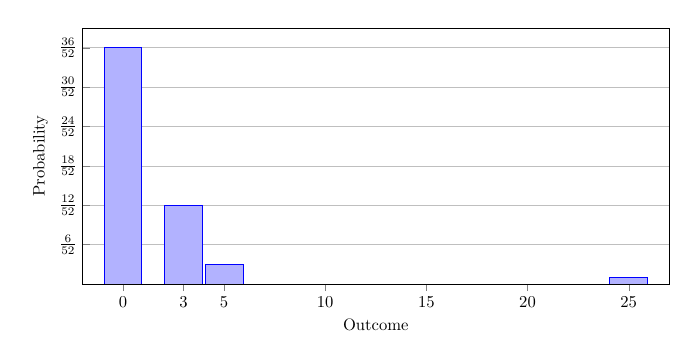
\begin{tikzpicture}[scale=0.6]
  \begin{axis}[ 
	ybar,
	xtick={0,3,5, 10, 15, 20, 25},
	ytick={6/52, 12/52, 18/52, 24/52, 30/52, 36/52},
	yticklabels={$\frac{6}{52}$,$\frac{12}{52}$,$\frac{18}{52}$,$\frac{24}{52}$,$\frac{30}{52}$,$\frac{36}{52}$},
	enlarge y limits=0,
	enlarge x limits=0,
	ymin=0,
	ymax=0.75,
  xmin=-2,
  xmax =27,
	xlabel=Outcome,
	ylabel=Probability,
    ymajorgrids=true,
	width=14cm,
	height=7cm,
  bar width=0.8cm,
	yticklabel style={
        /pgf/number format/fixed,
        /pgf/number format/precision=5
	},
	xtick pos=left,
	ytick pos=left,
	] 
  \addplot coordinates {
      (0, 36/52)
      (3, 12/52)
      (5, 3/52)
      (25, 1/52)
		};
  \end{axis}
\end{tikzpicture}

\end{center}

\end{solution}
\vfill
  \item
    Find the expected value of the game.
\begin{solution}
$$ 0 \left( \tfrac{36}{52} \right) + 3 \left( \tfrac{12}{52} \right) + 5 \left( \tfrac{3}{52} \right) + 25 \left( \tfrac{1}{52} \right) = \$ 1.461.$$
\end{solution}

\vfill
  \end{parts}

\setcounter{countA}{\value{question}}
\end{questions}

\subsubsection*{Random Variables}\label{random-variables}

When we use a letter to represent the numerical outcome of a probability
model, that letter is called a random variable. You should be
comfortable with the way random variables are used in notation, like
\(P(X > 5)\) for example.

\begin{questions}
\setcounter{question}{\value{countA}}

\item
  Suppose \(X\) is a \(N(500,80)\) random variable. Find the following.

  \begin{parts}
  \item
    \(P(X > 540)\)
\begin{solution}
Use the normal distributions app. 
$$P(X > 540) = 30.9\%.$$
\end{solution}
\vfill
  \item
    \(P(400 < X < 540)\)
\begin{solution}
$$P(400 < X < 540) = 100 - 10.6\% - 30.9\% = 58.5\%.$$
\end{solution}
\vfill
  \end{parts}

\setcounter{countA}{\value{question}}
\end{questions}

\subsubsection*{Sampling Distributions}\label{sampling-distributions}

Make sure you know the shape, center, and spread for the sampling
distributions of the sample mean \(\bar{x}\) and the sample proportion
\(\hat{p}\). Be sure you can describe how they change as the sample size
gets larger.

\begin{questions}
\setcounter{question}{\value{countA}}

\item
  Data collected by the Substance Abuse and Mental Health Services
  Administration (SAMSHA) suggests that 69.7\% of 18-20 year olds
  consumed alcoholic beverages in any given year. Suppose we consider a
  random sample of fifty 18-20 year olds.

  \begin{parts}
  \item
    Describe the sampling distribution for the proportion of students in the sample that have
    consumed alcoholic beverages in the past year. What is the shape,
    center, and spread of the distribution?
\begin{solution}
\begin{description}
\item[Shape] The shape will be approximately normal.
\item[Center] The center is 69.7\%.
\item[Spread] The spread is the standard deviation for $\hat{p}$:
$$\sigma_{\hat{p}} = \sqrt{\frac{p(1-p)}{N}} = \sqrt{\frac{0.697(1 - 0.697)}{50}} = 6.5\%.$$
\end{description}
\end{solution}
\vfill
  \item
    Estimate the probability that at least 80\% of the individuals in
    the sample have consumed alcohol in the past year.
\begin{solution}
Use the normal distributions app to find
$$P(X \ge 80\%) = 5.7\%.$$
\end{solution}
\vfill
  \end{parts}
\item
  (\href{http://people.hsc.edu/faculty-staff/blins/books/OpenIntroStats4e.pdf\#eoce.5.1}{Exercise 5.1 from OpenIntro Statistics}) For each of the following situations, state whether the
  parameter of interest is a mean or a proportion. It may be helpful to
  examine whether individual responses are numerical or categorical.

  \begin{parts}
  \item
    In a survey, one hundred college students are asked how many hours
    per week they spend on the Internet.
\begin{solution}
Mean (response is numerical)
\end{solution}
\vfill
  \item
    In a survey, one hundred college students are asked: ``What
    percentage of the time you spend on the Internet is part of your
    course work?''
\begin{solution}
Mean (response is a percent, which is numerical)
\end{solution}
\vfill
  \item
    In a survey, one hundred college students are asked whether or not
    they cited information from Wikipedia in their papers.
\begin{solution}
Proportion (response is categorical)
\end{solution}
\vfill
  \item
    In a survey, one hundred college students are asked what percentage
    of their total weekly spending is on alcoholic beverages.
\begin{solution}
Mean (response is numerical)
\end{solution}
\vfill
  \item
    In a sample of one hundred recent college graduates, it is found
    that 85 percent expect to get a job within one year of their
    graduation date.
\begin{solution}
Proportion (response is categorical: expect to have a job or not?)
\end{solution}
\vfill
  \end{parts}
\item
  As part of a quality control process for computer chips, an engineer
  at a factory randomly samples 212 chips during a week of production to
  test the current rate of chips with severe defects. She finds that 27
  of the chips are defective.

  \begin{parts}
  \item
    What population is under consideration in the data set?
\begin{solution}
All the chips produced at the facility.
\end{solution}
\vfill
  \item
    What parameter is being estimated?
\begin{solution}
The proportion of all chips with severe defects. 
\end{solution}
\vfill
  \item
    What is the best guess estimate for the parameter?
\begin{solution}
The sample proportion
$$\hat{p} = \frac{ 27 }{~ 212 ~} = 12.7\%.$$
\end{solution}
\vfill
  \item
    Calculate the standard error $\displaystyle \operatorname{SE}_{\hat{p}} = \sqrt{\frac{\hat{p}(1-\hat{p})}{N}}.$
\begin{solution}
$$\operatorname{SE}_{\hat{p}} = \sqrt{\frac{ 0.127 (1-0.127) }{ 212 }} = 2.29\%.$$
\end{solution}
\vfill
  \item
    The historical rate of defects is 10\%. Should the engineer be
    surprised by the observed rate of defects during the current week?
\begin{solution}
The rate of defects (12.7\%) is only a little more than one standard deviation (2.29\%) above the historical rate of defects, so that is not a surprising result. 
\end{solution}
\vfill
  \end{parts}
\item
  American adults have an average weight of \(170\) lbs. with a standard
  deviation of 40 lbs.

  \begin{parts}
  \item
    Describe the sampling distribution for the average weight of a
    random group of 25 adults.
\begin{solution}
\begin{description}
\item[Shape] The shape is approximately normal.
\item[Center] $\mu = 170$ lbs.
\item[Spread] The standard deviation of $\bar{x}$:
$$\sigma_{\bar{x}} = \frac{\sigma}{\sqrt{N}} = \frac{40}{\sqrt{25}} = 8 \text{ lbs}.$$
\end{description}
\end{solution}
\vfill
  \item
    Estimate \(P(\bar{x} > 180)\) using the normal distribution.
\begin{solution}
$$P(\bar{x} > 180) = 10.6\%.$$
\end{solution}
\vfill
  \end{parts}

\setcounter{countA}{\value{question}}
\end{questions}

\subsubsection*{Confidence Intervals for Proportions}
Make sure you understand that the confidence interval is a tool to estimate the population proportion $p$ using the sample proportion $\hat{p}$.  The confidence level is how confident we are that the true value of $p$ is inside the interval. 

\begin{questions}
\setcounter{question}{\value{countA}}

\question (\href{https://people.hsc.edu/faculty-staff/blins/books/OpenIntroStats4e.pdf#eoce.6.45}{Exercise 6.45 from OpenIntro Statistics}) We are interested in estimating the proportion of graduates at a mid-sized university who found a job within one year of completing their undergraduate degree. Suppose we conduct a
survey and find out that 348 of the 400 randomly sampled graduates found jobs. The graduating class under
consideration included over 4500 students.
\begin{parts}
\part Describe the population parameter of interest. What is the value of the point estimate of this parameter?
\begin{solution}
The parameter of interest is the percent of all graduates at the university who found a job within one year.  The best guess (point estimate) is $\hat{p} = \frac{348}{400} = 87\%$.
\end{solution}
\vfill
\part Check if the conditions for constructing a confidence interval based on these data are met.
\begin{solution}
The graduates were randomly sampled, which means we can hope that there was no bias. And there were 348 successes and 52 failures, so both are large enough to assume normality.
\end{solution}
\vfill
\part Calculate a 95\% confidence interval for the proportion of graduates who found a job within one year of completing their undergraduate degree at this university, and interpret it in the context of the data.
\begin{solution}
$$87\% \pm 1.96 \sqrt{\frac{0.87(1-0.87)}{400}} = 87\% \pm 3.3\%.$$
So we can be 95\% sure that the percent of graduates who found jobs within one year is between 83.7\% and 90.3\%. 
\end{solution}
\vfill
\part What does “95\% confidence” mean?
\begin{solution}
It means we can be 95\% sure that the confidence interval contains the parameter of interest. 
\end{solution}

\vfill
\part Now calculate a 99\% confidence interval for the same parameter and interpret it in the context of the data.
\begin{solution}
$$87\% \pm 2.576 \sqrt{\frac{0.87(1-0.87)}{400}} = 87\% \pm 4.3\%.$$
So we can be 99\% sure that the percent of graduates who found jobs within one year is between 82.7\% and 91.3\%. 
\end{solution}
\vfill
\part Which has a larger margin of error, the 95\% or the 99\% confidence interval?
\begin{solution}
The 99\% confidence interval has a larger margin of error. 
\end{solution}
\vfill
\end{parts}

\setcounter{countA}{\value{question}}
\end{questions}

\end{document}
